\documentclass{article}

\usepackage{neurips_2024}

\usepackage[T1]{fontenc}
\usepackage{hyperref}
\usepackage{url}
\usepackage{booktabs}
\usepackage{amsmath}
\usepackage{amssymb}
\usepackage{amsthm}
\usepackage{graphicx}
\usepackage{microtype}
\usepackage[capitalize,noabbrev]{cleveref}
\crefformat{equation}{(#2#1#3)}

\newtheorem{lemma}{Lemma}
\newtheorem{conjecture}{Conjecture}
\newtheorem{fact}{Fact}
\crefname{lemma}{Lemma}{Lemmas}
\crefname{conjecture}{Conjecture}{Conjectures}
\crefname{fact}{Fact}{Facts}
\crefname{table}{Table}{Tables}

\DeclareMathOperator{\End}{End}
\newcommand{\SU}{\mathrm{SU}}
\newcommand{\SO}{\mathrm{SO}}
\newcommand{\PSU}{\mathrm{PSU}}
\newcommand{\Spin}{\mathrm{Spin}}
\newcommand{\PSO}{\mathrm{PSO}}
\newcommand{\Sp}{\mathrm{Sp}}
\newcommand{\R}{\mathbb{R}}
\newcommand{\C}{\mathbb{C}}
\newcommand{\HH}{\mathbb{H}}
\newcommand{\Z}{\mathbb{Z}}

\title{Neural networks trained on compact group composition\\
learn the global form of the group}

\author{Anonymous}

\begin{document}

\maketitle

\begin{abstract}
Small neural networks trained to identify products in a compact Lie group
learn the irreducible representations of the group. Across ten group forms
drawn from $\SU(2)$, $\SU(3)$, $\Spin(4)$, and $\Spin(5)$ and their central
quotients, with each element presented through a fixed generic encoding,
the trained features concentrate on the matrix coefficients of a small
faithful representation of the task group, the same one in every seed, and
half-integer spins appear precisely when the encoding distinguishes the two
sheets of the double cover. The learned features therefore determine the
isomorphism type of the group and not merely its Lie algebra. Ablations
show that each isotypic component is necessary for exactly the center
discriminations its central character supports. A test based on the
two-sided translation action shows that the features span the full
matrix-coefficient space of the representation, whose real dimension the
real Schur lemma prescribes, and that they admit commuting linear left and
right translation actions. A frame of two columns of a rotation matrix
determines the rotation with fewer coordinates and admits a linear left
action, yet in matched training on $\SO(3)$ the $9$-dimensional
coefficient space attains a larger margin than the $6$-dimensional frame
at $17\%$ lower total parameter norm, so regularized training selects the
coefficient space as the cheaper complete mechanism. Under regression onto
heat-kernel targets, the same architecture fills isotypic components in
order of Casimir eigenvalue up to a truncation point that moves with the
weight decay. One finding is negative. On $\SO(5)$, a stable
vector-plus-adjoint mixture survives every replication, so the
minimal-representation description fails as stated in one of the ten
group forms.
\end{abstract}

\section{Introduction}

By the Peter--Weyl theorem, the matrix coefficients of the irreducible
unitary representations of a compact Lie group span a dense subspace of
$L^2$ of the group \cite[Ch.~III]{brocker1985}. For \emph{finite} groups,
mechanistic interpretability has established that small networks trained
on the multiplication table represent elements through matrix coefficients
of a few irreducible representations \cite[Sec.~4]{chughtai2023}, that
competing descriptions of the same models exist
\cite[Sec.~5]{stander2024}, and that per-argument equivariance reconciles
them \cite{wu2024}. All of this work presupposes a finite table and one
learned embedding per element, the setting of the grokking literature
\cite{power2022, nanda2023, gromov2023, zhong2023}, the associated theory
proves emergence of irreducible features for finite groups
\cite{morwani2024, marchetti2024}, and equivariant architectures build the
harmonics into the network \cite{cohen2016, geiger2022}. Whether this
representation theory emerges in a generic network when the group is a
continuum has remained open.

In this paper, we answer that question and report the regularities that
the analysis uncovered along the way. We train encoder-factorized scorers
to identify products in compact groups, with each element presented
through a fixed generic encoding, and we analyze the learned features by
isotypic decomposition, ablation, activation patching, and a test built on
the two-sided translation action of the group on its own matrix
coefficients. Four findings result, and the last revises the first.

\textbf{The learned representation determines the global form of the
group.} For each central subgroup $Z \subseteq Z(G)$, averaging the
encoding over $Z$ realizes the same task on the quotient $G/Z$, so the
isomorphism type of the group becomes an experimental variable while the
Lie algebra stays fixed. Across ten group forms (\cref{tab:carriers}), the
trained features concentrate $93$--$98\%$ of their variance on the matrix
coefficients of a small faithful representation of the task group, the
same one in every seed, and every isotypic component that the descent rule
forbids stays at the measurement floor. The selection is causal. Ablating
the learned representation collapses ranking to chance and removes exactly
the center discriminations its central character supports, while
equal-rank ablations elsewhere leave the model intact
(\cref{sec:carriers}).

\textbf{The learned features span the full matrix-coefficient space, and
cost selects it.} The active subspace of the features has exactly the real
dimension $(\dim_\R W)^2/\dim_\R \End_G(W)$ of the full coefficient space
of the learned representation $W$, and fitted left and right translation
operators reach held-out $R^2 \geq 0.98$ and commute, which characterizes
the full coefficient space inside its isotypic component
(\cref{lem:twosided}). A frame of two columns determines a rotation with
six coordinates and admits an exactly linear left action, and its right
action fails to be linear. In matched training on $\SO(3)$, the
$9$-dimensional coefficient space attains a larger margin than the
$6$-dimensional frame at $17\%$ lower parameter norm (\cref{sec:block}).
Regularized training selects the coefficient space because composition and
scoring become bilinear on it, and the saving on those maps exceeds the
cost of the extra coordinates.

\textbf{Regression targets reveal a spectral bias ordered by the Casimir
eigenvalue.} Trained to regress heat-kernel values $K_t(ab\,c^{-1})$, the
same architecture recovers the required isotypic components at their
required weights up to a sharp truncation point, the truncation advances
in order of Casimir eigenvalue during training, in analogy with the
spectral bias of \cite{rahaman2019}, and the truncation moves with the
regularization strength. On a band-limited target, weight decay $1.0$
prunes an in-support component that weight decay $0.1$ retains
(\cref{sec:spectral}).

\textbf{One finding is negative.} On $\SO(5)$, a stable
vector-plus-adjoint mixture survives five seeds and every conditioning
variation we ran, so the minimal-representation description fails as
stated in one of ten group forms. We report the failure in
\cref{sec:limits} together with the two hypotheses that remain open.

Our analysis methods are standard. The new ingredients are the object, a
continuum group with no embedding table, the quotient construction that
turns the isomorphism type into an experimental variable, and the
two-sided translation test of \cref{sec:block}. The rest of this paper is
organized as follows. In \cref{sec:setup}, we fix the task and the
analysis methods. In \cref{sec:carriers,sec:block,sec:spectral}, we
present the three positive findings. In \cref{sec:limits}, we present the
negative finding and a selection conjecture. Background from
representation theory and harmonic analysis is collected in
\cref{app:background}, proofs are in \cref{app:proofs}, experimental
details in \cref{app:details}, and complete result tables and additional
figures in \cref{app:tables}.

\section{Task, encodings, and analysis methods}
\label{sec:setup}

Throughout, $G$ denotes a compact Lie group with Haar probability measure,
$Z \subseteq Z(G)$ a central subgroup, $W$ an irreducible real
representation of $G$ with commutant $\End_G(W) \in \{\R, \C, \HH\}$,
$z(g) \in \R^{128}$ the trained argument-encoder activations, and
$\chi_\rho$ the character of an irreducible unitary representation $\rho$.

\textbf{Task.} Given encodings of $a, b \in G$ and of $K = 64$ candidates,
the model must identify the product. The positive candidate is
$(ab)\exp(\xi)$ with $\xi$ a centered Gaussian of scale $\sigma = 0.2$ on
the Lie algebra, the $K - 1$ negatives are Haar samples excluded from a
ball around the positive class, and the loss is cross-entropy over the $K$
scores. The Bayes-optimal rule ranks candidates by distance to $ab$ and
attains accuracy $0.951$ under the $\SU(2)$ sampling. Training pairs come
from a pool of $2048$ Haar elements, and we report ranking accuracy on
pairs of fresh elements never seen in training.

\textbf{Encodings.} Each element enters through a fixed map $\Psi$, so the
model has no per-element parameters. For $\SU(2)$, we take
$\Psi(q)_i = \exp(\alpha \langle q, h_i\rangle)$ with $32$ fixed Haar
landmarks $h_i$ and $\alpha = 3$, standardized under Haar statistics. The
quotient condition for $G/Z$ replaces $\Psi$ by its average over the
$Z$-orbit. The averaged map is exactly $Z$-invariant and separates the
elements of $G/Z$, so it realizes the quotient group, and the two
conditions share landmarks, dimension, and all hyperparameters. Every
result below reproduces under two further encodings (\cref{app:details}),
so the selected representation is a property of the task and the group.

\textbf{Model.} An encoder-factorized scorer with about $0.3$M parameters.
A shared two-layer GELU encoder produces $z(a), z(b)$, an interaction
network produces $h(a,b) \in \R^{128}$, a candidate encoder produces
$z_c(c)$, and the score is $\langle h(a,b), z_c(c)\rangle$, trained by
AdamW with weight decay $1.0$ unless stated. Every reported quantity is a
mean over five seeds with its standard deviation.

\textbf{Analysis methods.} The isotypic decomposition computes, on a fixed
Haar probe set, the fraction of variance of the centered activations $z$
lying in the sampled, jointly orthonormalized spans of matrix
coefficients, component by component in order of Casimir eigenvalue, with
exact coefficients verified in a unit-test suite (\cref{app:details}) and
a sampling floor near $0.2\%$ of variance. Ablations subtract from $z$ the
part linearly predictable from a chosen component's exact matrix
coefficients, an intervention well defined even for components at the
floor. Activation patching replaces the internal product state by
reconstructions from chosen coordinates. The activations are real, so a
complex irreducible representation and its conjugate span one real
isotypic component, of dimension $(\dim_\R W)^2 / \dim_\R \End_G(W)$
(\cref{lem:twosided}, with background in \cref{app:background}).

\section{The learned representation determines the global form}
\label{sec:carriers}

\begin{figure}[t]
\centering
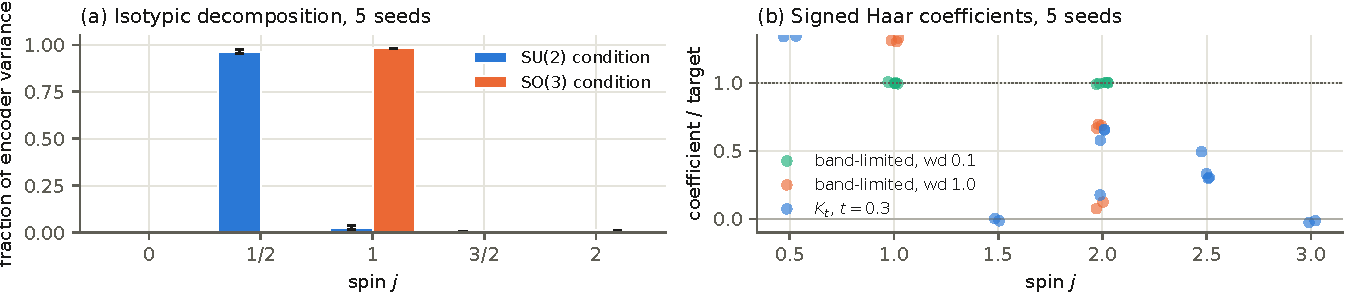
\includegraphics[width=0.92\textwidth]{figure1.pdf}
\caption{(a) Isotypic decomposition of the trained encoder for the
$\SU(2)$ and $\SO(3)$ conditions (five seeds). (b) Recovery of the
character expansion of the score for heat-kernel and band-limited targets.
Values near $1$ indicate a component carried at its required weight, and
the dashed curve shows the in-support spin-$2$ component pruned at weight
decay $1.0$.}
\label{fig:main}
\end{figure}

\begin{table}[t]
\centering
\caption{Learned representations across ten group forms, with the fraction
of encoder variance on their matrix coefficients (mean over five seeds)
and the rejected faithful alternative where one exists. $\Spin(4)$
representations are labeled by pairs $(j_L, j_R)$. Seed statistics and
intervention results per condition are in \cref{app:tables}.}
\label{tab:carriers}
\small
\setlength{\tabcolsep}{5pt}
\begin{tabular}{llll}
\toprule
task group & learned representation & variance & rejected alternative \\
\midrule
$\SU(2)$ & spin $\tfrac12$ & $0.96$ & \\
$\SO(3)$ & spin $1$ & $0.98$ & \\
$\SU(3)$ & $\mathbf{3} \oplus \bar{\mathbf{3}}$ & $0.97$ & \\
$\PSU(3)$ & adjoint $\mathbf{8}$ & $0.93$ & \\
$\Spin(4)$ & $(\tfrac12,0) \oplus (0,\tfrac12)$ & $0.98$ & (no faithful irreducible) \\
$\SO(4)$ & $(\tfrac12,\tfrac12)$ & $0.97$ & \\
$\SO(3){\times}\SU(2)$ & $(1,0) \oplus (0,\tfrac12)$, $5$ dims & $0.98$ & $(1,\tfrac12)$, $6$ dims: $0.008$ \\
$\PSO(4)$ & $(1,0) \oplus (0,1)$, $6$ dims & $0.98$ & $(1,1)$, $9$ dims: $0.011$ \\
$\Spin(5)$ & spinor $\mathbf{4}$ & $0.97$ & \\
$\SO(5)$ & vector $\mathbf{5}$ + adjoint $\mathbf{10}$ & $0.69 + 0.22$ & (see \cref{sec:limits}) \\
\bottomrule
\end{tabular}
\end{table}

Across the ten group forms of \cref{tab:carriers}, the trained features
concentrate on the matrix coefficients of a small faithful representation
of the task group, the same one in every seed. The half-integer component
of $\SU(2)$ appears if and only if the encoding distinguishes $\pm g$,
with $\cos(z(g), z(-g)) = -0.95 \pm 0.02$ in the faithful condition and
$+1.000$ in the quotient condition. The learned features therefore detect
the double cover, a property of the isomorphism type that the Lie algebra
does not determine. When the center of the group fails to be cyclic, no
faithful irreducible representation exists (\cref{fact:cyclic}), and the
models build the direct sum that faithfulness forces. Where a smaller
reducible faithful sum competes against a larger faithful irreducible
representation, the sum wins, with the alternative under $1\%$ of variance
in every seed.

The selection is causal. Subtracting from $z$ the part linearly
predictable from the learned representation's matrix coefficients
collapses ranking to chance ($0.02$ against a chance rate of $0.016$) and
collapses center discrimination to its tie value, while the same ablation
on any other component, or on a random subspace of equal rank, leaves both
intact. The pattern is a double dissociation between each group and its
quotient, with seed standard deviations below $0.005$ on every cell
(\cref{tab:su2causal}). It repeats under the order-three center of
$\SU(3)$, where orbit averaging acts as the identity on quotient models
and destroys the faithful ones (\cref{tab:su3causal}), and it holds
summand by summand for $\Spin(4)$, whose center supports three distinct
discriminations, with each learned summand necessary for exactly the
center elements its central character detects (\cref{tab:spin4causal}).
The trained scorer is itself a character function, and a single character
explains $0.97 \pm 0.01$ of the score variance for $\SU(2)$ (with
$\chi_{1/2}$) and $0.88 \pm 0.01$ for $\SO(3)$ (with $\chi_1$).

The following bound, proved in \cref{app:proofs}, explains why ranking
never forces a larger representation.

\begin{lemma}
\label{lem:character}
Let $V$ be a faithful finite-dimensional unitary representation of a
compact group $H$ with character $\chi_V$. Then
$\operatorname{Re}\chi_V(g) \leq \chi_V(e)$ for all $g \in H$, with
equality only at $g = e$. Moreover, for $X$ in the Lie algebra of $H$,
$\operatorname{Re}\chi_V(\exp X) = \chi_V(e) -
\tfrac12 \lVert dV(X)\rVert_{F}^2 + O(\lVert X\rVert^4)$,
and $X \mapsto \lVert dV(X)\rVert_F^2$ is positive definite.
\end{lemma}

By \cref{lem:character}, a monotone function of
$\operatorname{Re}\chi_V(ab\,c^{-1})$ ranks the product above every
excluded negative for any faithful $V$, so optimization selects the
representation on cost. Conversely, a representation with nontrivial
kernel forces positive ranking error under explicit sampling assumptions
(\cref{lem:necessity}), and the ablations above realize that necessity
summand by summand.

\section{The learned features span the full coefficient space}
\label{sec:block}

The learned features occupy their isotypic component fully. In every seed,
the active subspace of $z$ has exactly the real dimension of the full
coefficient space, $4$ for the quaternionic spinor and $9$ for the
real-type vector representation, as the following lemma prescribes (proof
in \cref{app:proofs}).

\begin{lemma}
\label{lem:twosided}
Let $\rho \colon G \to U(V_\rho)$ be an irreducible unitary representation
of a compact group $G$, and let $M_\rho \subseteq L^2(G)$ be the span of
its matrix coefficients $g \mapsto \langle u, \rho(g) v\rangle$. Then
$M_\rho \cong V_\rho^* \boxtimes V_\rho$ as a representation of
$G \times G$ acting by left and right translation, this representation is
irreducible, and every nonzero subspace of $M_\rho$ invariant under both
translation actions equals $M_\rho$. For an irreducible real
representation $W$ with commutant $D = \End_G(W)$, the corresponding real
coefficient space has dimension $(\dim_\R W)^2 / \dim_\R D$ and is the
minimal nonzero two-sided translation-stable real subspace of its isotypic
component.
\end{lemma}

\textbf{Two-sided structure.} \Cref{lem:twosided} makes full-coefficient
identity falsifiable. The full coefficient space admits commuting linear
left and right translation actions, and every proper subspace of the
isotypic component loses at least one of them. We fit affine operators
$M^L_k$, $M^R_k$ with $z(kg) \approx M^L_k z(g)$,
$z(gk) \approx M^R_k z(g)$, evaluated held out. On the trained $\SO(3)$
features, both actions fit at $R^2 = 0.989 \pm 0.001$ with relative
commutator defect $\lVert [M^L_a, M^R_b]\rVert = 0.012 \pm 0.001$,
matching the exact coefficient space. On the frame
$g \mapsto (g e_1, g e_2)$, the left action is exactly linear and the
right action fits at $R^2 = 0.638$, since the missing column
$g e_3 = (g e_1) \times (g e_2)$ is uncorrelated with the retained ones
under Haar measure. A random subspace of the coefficient space at the
frame's dimension loses both actions, fitting at $R^2 = 0.67$ (full
comparison in \cref{tab:twosided}). The fitted operators realize the
representation itself. The trace of $M^L_k$ equals
$\dim(W)\,\chi_W(k)$ with correlation $1.000$ across group elements, and
its eigenvalue phases match those of $\dim(W)$ copies of $W(k)$ to
$0.002$ radians for $\SU(2)$.

\textbf{Causal sufficiency.} Replacing the internal product state $h(a,b)$
by its ridge reconstruction from the eight realified spinor coefficients
of a counterfactual product $a'b'$ redirects the $\SU(2)$ model to select
$a'b'$ with probability $0.996$--$0.999$ in every seed, equal to or better
than patching the full activation, while reconstruction from the wrong
component redirects at chance. The output $h$ concentrates
$89.9 \pm 1.4\%$ of its variance on the diagonal two-argument component of
the learned representation, with $98.2 \pm 0.3\%$ of that energy in the
subspace spanned by the matrix product $W(a)W(b)$, so the interaction
network implements the representation's own composition law.

\textbf{Cost.} To test whether two-sided linearity is the reason the
coefficient space wins, we trained matched models on $\SO(3)$ whose
encodings are the exact frame with $6$ coordinates or the exact
coefficient space with $9$, all else equal. At statistically equal
accuracy ($0.891 \pm 0.002$ against $0.889 \pm 0.003$), the
coefficient-space model attains a larger margin ($7.29 \pm 0.16$ against
$6.49 \pm 0.05$) at $17\%$ lower total parameter norm, with every module
cheaper (\cref{tab:cost}). The frame model reconstructs the missing column
nonlinearly, and the reconstruction costs more than the three saved
coordinates. Regularized training therefore selects the full coefficient
space as the cheapest complete mechanism, with storage and composition
counted together.

\section{Spectral bias in order of the Casimir eigenvalue}
\label{sec:spectral}

Ranking requires a single faithful character, so it leaves the allocation
of capacity across isotypic components unobserved. Regression onto the
$\SU(2)$ heat kernel $K_t(g) = \sum_j (2j+1) e^{-t\,j(j+1)} \chi_j(g)$,
evaluated at $ab\,c^{-1}$, requires every component that the envelope
keeps above the noise. \Cref{fig:main}(b) reports the fraction of score
variance per component, sequentially orthogonalized in order of Casimir
eigenvalue, divided by the same fraction for the exact target, so a value
of $1$ means a component at its required weight (per-checkpoint values in
\cref{tab:recovery}).

Three regularities emerge. First, each trained score is a truncated
character expansion, with recovered components near ratio $1$, components
beyond a sharp truncation point at $0$, and the truncation at higher
Casimir eigenvalue for smaller $t$. Second, the truncation advances in
order of Casimir eigenvalue during training. At $t = 0.05$, the spin-$2$
recovery climbs from $0.12$ to $1.20$ over $70$k steps while spin
$\tfrac52$ stays at $0$. Third, the truncation moves with the
regularization strength. On the band-limited target
$\chi_1 + \tfrac12 \chi_2$, weight decay $1.0$ prunes the spin-$2$ part,
the abandoned $12.6\%$ of target variance equals the final test error, and
weight decay $0.1$ recovers the target with profile
$(1.00, 1.01, 0.94, 0.95)$ and out-of-support components at $0.000$. A
component survives when its variance contribution exceeds its norm cost,
so the truncation is a cost boundary of the same kind that selects the
representation in \cref{sec:carriers}. The central character of the target
governs the parity of the learned features as well. The band-limited
target is invariant under the center, and the model builds an integer-spin
representation even on the faithful $\SU(2)$ encoding, with the spinor
component at $1\%$.

\section{A negative finding, and a selection conjecture}
\label{sec:limits}

On $\SO(5)$, the learned features occupy a mixture, the vector
$\mathbf{5}$ at $0.68$--$0.70$ of variance and the adjoint $\mathbf{10}$
at $0.21$--$0.23$, stable across five seeds, doubled training, four times
the candidates, and reduced weight decay. The adjoint fraction falls only
when generalization improves, from $0.23$ at held-out accuracy $0.55$ to
$0.17$ at $0.73$ under tripled data, and no condition solves the task. The
minimal-representation description therefore fails as stated in one of the
ten group forms. Both faithful components ranking correctly is consistent
with \cref{lem:character}, and two hypotheses remain open, purification as
the task approaches a solution, or a genuinely mixed minimum-cost
mechanism for this group, which the cost result of \cref{sec:block} makes
coherent. Separating them requires a condition that solves $\SO(5)$.

The structural results suggest a selection principle that we can state but
cannot yet prove.

\begin{conjecture}
In the factorized architecture with weight decay, among parameter settings
achieving population ranking loss within $\varepsilon$ of the optimum, the
minimum-norm setting realizes, as $\varepsilon \to 0$, the full real
coefficient space of a faithful representation minimizing the total
regularized cost of features, composition, and scoring, with score a
monotone function of $\operatorname{Re}\chi_V(ab\,c^{-1})$.
\end{conjecture}

The missing ingredients are a norm lower bound tying any
$\varepsilon$-optimal score to the effective dimension of the functions it
computes on $G$, and the exclusion of solutions outside the character
algebra, the compact-group analogue of the alternative circuits documented
for finite groups \cite{stander2024, zhong2023}. Every quotient condition
in our experiments generalizes below its cover, and disentangling
representation selection from the conditioning of the quotient encoding is
left as future work.

\bibliographystyle{unsrtnat}
\bibliography{refs}

\appendix

\section{Background: representation theory and harmonic analysis on compact groups}
\label{app:background}

This appendix collects the facts the paper uses, with references in place
of proofs. Standard sources are \cite{brocker1985} for compact groups and
the Peter--Weyl theorem, \cite{sepanski2007} for the real Schur lemma and
the type classification, \cite{folland1995} for harmonic analysis, and
\cite{fulton1991} for the representation theory of the classical groups.
Throughout, $G$ is a compact Lie group and all representations are
finite-dimensional and continuous.

\paragraph{Haar measure and unitarity.}
A compact group carries a unique translation-invariant Borel probability
measure, its Haar measure, and every expectation over group elements in
this paper is taken with respect to it. Averaging an arbitrary inner
product over the group makes any representation unitary, and every unitary
representation decomposes as a finite orthogonal direct sum of irreducible
ones \cite[Ch.~II]{brocker1985}. The set of isomorphism classes of complex
irreducible representations is denoted $\widehat G$, and for
$\rho \in \widehat G$ we write $d_\rho = \dim V_\rho$ and
$\chi_\rho(g) = \operatorname{tr}\rho(g)$ for its character.

\paragraph{Matrix coefficients and orthogonality.}
For $\rho \in \widehat G$ and vectors $u, v \in V_\rho$, the function
$g \mapsto \langle u, \rho(g) v\rangle$ is a matrix coefficient of $\rho$.
Schur's lemma states that a linear map commuting with two irreducible
representations is zero or an isomorphism, and that the self-intertwiners
of a complex irreducible representation are the scalars
\cite[Ch.~I]{fulton1991}. Its integrated form is the orthogonality of
coefficients. In a unitary basis,
\[
\int_G \rho(g)_{ij}\, \overline{\sigma(g)_{kl}}\, dg
\;=\; \frac{\delta_{\rho\sigma}\,\delta_{ik}\,\delta_{jl}}{d_\rho},
\qquad
\int_G \chi_\rho(g)\, \overline{\chi_\sigma(g)}\, dg
\;=\; \delta_{\rho\sigma}
\]
for $\rho, \sigma \in \widehat G$ \cite[Ch.~II]{brocker1985}. These
relations underlie the isotypic decomposition of \cref{sec:setup}. They
make the coefficient spans of distinct irreducible representations
orthogonal in $L^2(G)$, so variance fractions per component are well
defined, and our implementation verifies them numerically on the sampled
probe sets.

\paragraph{The Peter--Weyl theorem.}
The matrix coefficients of all $\rho \in \widehat G$ span a dense subspace
of $L^2(G)$, and as a representation of $G \times G$ acting by left and
right translation,
\[
L^2(G) \;\cong\; \bigoplus_{\rho \in \widehat G} M_\rho,
\qquad M_\rho \;\cong\; V_\rho^* \boxtimes V_\rho,
\]
an orthogonal Hilbert-space direct sum in which each coefficient space
$M_\rho$ has dimension $d_\rho^2$ \cite[Ch.~III]{brocker1985}. Every
function a network computes on $G$ therefore has a spectral decomposition
over $\widehat G$, and the structural question of this paper, which
components a trained model occupies and whether it occupies them fully, is
a question about this decomposition. \Cref{lem:twosided} records the
two-sided irreducibility of $M_\rho$ and its real form.

\paragraph{Real representations and Schur type.}
The networks compute with real numbers, so the relevant decomposition is
that of real representations. For an irreducible real representation $W$,
the real Schur lemma states that the commutant $\End_G(W)$ is a real
division algebra, hence isomorphic to $\R$, $\C$, or $\HH$
\cite[Ch.~III]{sepanski2007}, and the three cases correspond to the
classical trichotomy for a complex irreducible representation $V$. The
representation $V$ has real type when it admits an invariant real
structure, quaternionic type when it admits an invariant quaternionic
structure, and complex type when $V \not\cong \bar V$. Realification acts
on dimensions as follows. A real-type $V$ of dimension $d$ yields
$\dim_\R W = d$ with commutant $\R$. A complex-type or quaternionic-type
$V$ of dimension $d$ yields $\dim_\R W = 2d$ with commutant $\C$ or $\HH$,
and in the complex case $V$ and $\bar V$ realify to the same $W$, which is
why a complex irreducible representation and its conjugate span a single
real isotypic component in our measurements. In all three cases, the real
coefficient space has dimension
\[
\dim_\R M_W \;=\; \frac{(\dim_\R W)^2}{\dim_\R \End_G(W)},
\]
which evaluates to $d^2$, $2d^2$, and $d^2$ in the real, complex, and
quaternionic cases. The three dimensions measured in the paper are
instances, namely $9$ for the real-type vector representation of $\SO(3)$,
$18$ for the complex-type fundamental pair of $\SU(3)$, and $4$ for the
quaternionic spinor of $\SU(2)$.

\paragraph{Characters, class functions, and the scoring identity.}
Characters are conjugation-invariant, and the irreducible characters form
an orthonormal basis of the class functions in $L^2(G)$
\cite[Ch.~II]{brocker1985}. Two identities are used throughout, namely
$\chi_\rho(g^{-1}) = \overline{\chi_\rho(g)}$ and, for unitary $\rho$,
\[
\chi_\rho(ab\,c^{-1})
\;=\; \operatorname{tr}\bigl(\rho(a)\rho(b)\rho(c)^{*}\bigr)
\;=\; \bigl\langle \rho(c),\, \rho(a)\rho(b) \bigr\rangle_{\mathrm{HS}},
\]
so a character evaluated at $ab\,c^{-1}$ is a Hilbert--Schmidt pairing of
the candidate's coefficients against the product of the arguments'
coefficients. This identity supports the statement in \cref{sec:block}
that composition and scoring become bilinear on the coefficient space, and
it is the form in which the finite-group mechanism of \cite{chughtai2023}
extends to the compact case.

\paragraph{Central characters and descent to quotients.}
By Schur's lemma, the center $Z(G)$ acts in any $\rho \in \widehat G$ by a
character $\omega_\rho \colon Z(G) \to U(1)$, called the central
character. For a closed central subgroup $Z$, the irreducible
representations of the quotient $G/Z$ are exactly those $\rho$ with
$\omega_\rho$ trivial on $Z$, and the spectral support of a $Z$-invariant
function on $G$ consists of such $\rho$ alone. This is the descent rule of
\cref{sec:carriers}. The orbit-averaged encoding is $Z$-invariant, so
every component carrying a nontrivial central character of $Z$ is
forbidden, and the measured floors on those components are the empirical
form of the rule. One consequence used for $\Spin(4)$ deserves a proof,
since it forces the direct-sum representations of \cref{tab:carriers}.

\begin{fact}
\label{fact:cyclic}
If a compact group admits a faithful irreducible complex representation,
its center is isomorphic to a closed subgroup of $U(1)$. In particular,
$\Spin(4)$, with center $\Z_2 \times \Z_2$, has no faithful irreducible
representation.
\end{fact}

\begin{proof}
Under a faithful irreducible $\rho$, the center acts by the scalars
$\omega_\rho$, and faithfulness makes $z \mapsto \omega_\rho(z)$
injective, so $Z(G)$ embeds in $U(1)$. Every finite subgroup of $U(1)$ is
cyclic, and $\Z_2 \times \Z_2$ is not.
\end{proof}

\paragraph{The Casimir element and the heat kernel.}
Fix a bi-invariant metric on $G$. The quadratic Casimir element of the
universal enveloping algebra acts in each irreducible representation
$\rho$ as a scalar $C(\rho) \geq 0$, and the matrix coefficients of $\rho$
are eigenfunctions of the Laplace--Beltrami operator on $G$ with
eigenvalue $C(\rho)$ \cite[Ch.~5]{sepanski2007}. The Casimir eigenvalue
therefore plays the role of a squared frequency, and ordering components
by Casimir eigenvalue in this paper is the compact-group analogue of
ordering Fourier modes by frequency. The heat kernel at the identity-based
variable $g$ is the class function
\[
K_t(g) \;=\; \sum_{\rho \in \widehat G} d_\rho\, e^{-t\,C(\rho)}\,
\chi_\rho(g),
\]
the fundamental solution of the heat equation on $G$
\cite[Ch.~1]{folland1995}, and its envelope $e^{-t\,C(\rho)}$ determines
the required component weights in \cref{sec:spectral}.

\paragraph{The groups of the experiments.}
The irreducible representations of $\SU(2)$ are the spin representations
$D^j$ of dimension $2j+1$ for
$j \in \{0, \tfrac12, 1, \tfrac32, \dots\}$, with Casimir eigenvalue
$C(D^j) = j(j+1)$, quaternionic type for half-integer $j$ and real type
for integer $j$, and central character $(-1)^{2j}$ at $-1 \in \SU(2)$
\cite[Ch.~II]{brocker1985}. The quotient $\SO(3) = \SU(2)/\{\pm 1\}$
therefore carries exactly the integer spins, which yields the double-cover
diagnostic of \cref{sec:carriers}. The irreducible representations of
$\SU(3)$ are labeled by highest weights $(p, q)$ with dimension
$\tfrac12 (p+1)(q+1)(p+q+2)$ and central character $\omega^{\,p-q}$ at the
central element $\omega I$ for $\omega$ a primitive cube root of unity, so
descent to $\PSU(3)$ requires $p \equiv q \pmod 3$. The components tracked
in the experiments are the fundamental pair
$\mathbf{3} \oplus \bar{\mathbf{3}}$ at $(1,0)$ and $(0,1)$, the adjoint
$\mathbf{8}$ at $(1,1)$, and the pairs $\mathbf{6} \oplus \bar{\mathbf{6}}$
and $\mathbf{10} \oplus \bar{\mathbf{10}}$ \cite[Ch.~13]{fulton1991}. The
group $\Spin(4)$ is isomorphic to $\SU(2) \times \SU(2)$, its irreducible
representations are the outer products $(j_L, j_R)$ with central character
$\bigl((-1)^{2j_L}, (-1)^{2j_R}\bigr)$ on the center $\Z_2 \times \Z_2$,
and its three central quotients are $\SO(4)$ from the diagonal $\Z_2$,
retaining $j_L + j_R \in \Z$, the product $\SO(3) \times \SU(2)$ from one
factor's $\Z_2$, and $\PSO(4)$ from the full center, retaining
$j_L, j_R \in \Z$. The group $\Spin(5)$ is isomorphic to the quaternionic
unitary group $\Sp(2)$, with quaternionic spinor representation
$\mathbf{4}$, real vector representation $\mathbf{5}$, and adjoint
$\mathbf{10}$, and $\SO(5) = \Spin(5)/\{\pm 1\}$ retains the
representations with trivial central character, among them $\mathbf{5}$
and $\mathbf{10}$ \cite[Ch.~16]{fulton1991}.

\section{Proofs}
\label{app:proofs}

\begin{proof}[Proof of \cref{lem:character}]
Each eigenvalue of the unitary matrix $V(g)$ lies on the unit circle, so
$\operatorname{Re}\operatorname{tr} V(g) \leq \dim V$, with equality
exactly when every eigenvalue equals $1$, that is, when $V(g)$ is the
identity. By faithfulness, this occurs only at $g = e$. For the expansion,
write $A = dV(X)$, an anti-Hermitian matrix with eigenvalues
$i\lambda_1, \dots, i\lambda_{\dim V}$. Then
$\operatorname{Re}\operatorname{tr}\exp(tA) = \sum_k \cos(t\lambda_k) =
\dim V - \tfrac{t^2}{2}\sum_k \lambda_k^2 + O(t^4)$, and
$\sum_k \lambda_k^2 = \lVert A\rVert_F^2$. The trace of $A$ is purely
imaginary and contributes nothing to the real part. If
$\lVert dV(X)\rVert_F = 0$, then the one-parameter subgroup $\exp(tX)$
lies in the kernel of $V$, which is trivial, so $X = 0$, proving positive
definiteness.
\end{proof}

\begin{lemma}
\label{lem:necessity}
Let $H$ be a compact group. Assume the score factors as
$s(a,b,c) = S(\varphi(a), \varphi(b), \varphi(c))$ where $\varphi$ factors
through the matrix coefficients of a representation $V$ of $H$ with
nontrivial closed kernel $N$, the function $c \mapsto s(a,b,c)$ is
continuous, negatives are sampled from a distribution assigning positive
probability to every open subset of the admissible region, and the
exclusion radius is smaller than $\min_{n \in N,\, n \neq e} d(e, n)$.
Then the population ranking loss is bounded away from its optimum.
\end{lemma}

\begin{proof}
Fix $n \in N$ with $n \neq e$. By the radius hypothesis, $ab\,n$ lies in
the admissible negative region. Since $\varphi$ is constant on $N$-cosets,
$s(a, b, ab\,n) = s(a, b, ab)$, which is at least the score of the noisy
positive up to the continuity modulus of $s$ over the positive
displacement. By continuity, there is a ball around $ab\,n$ on which the
score stays within any prescribed gap of this value, and by the sampling
hypothesis that ball receives positive probability, so with positive
probability a sampled negative ties or exceeds the positive.
\end{proof}

The hypotheses of \cref{lem:necessity} are needed. With a finite kernel
and a continuous candidate distribution, the exact ambiguous points have
measure zero, and without continuity of the score no positive lower bound
follows from non-separation alone.

\begin{proof}[Proof of \cref{lem:twosided}]
The map $V_\rho^* \otimes V_\rho \to L^2(G)$ sending $u^* \otimes v$ to
$g \mapsto \langle u, \rho(g) v \rangle$ intertwines the
$G \times G$-action by left and right translation with the outer tensor
product action and is injective by the orthogonality of matrix
coefficients (\cref{app:background}). The outer tensor product of
irreducible representations is an irreducible representation of the
product group, so $M_\rho$ has no proper nonzero two-sided invariant
subspace, and $\dim_\C M_\rho = (\dim V_\rho)^2$. For the real form, the
real Schur lemma gives $\End_G(W) \in \{\R, \C, \HH\}$, and the real
matrix-coefficient span of $W$ is identified with $W^* \otimes_{D} W$, of
real dimension $(\dim_\R W)^2/\dim_\R D$. Minimality follows from
irreducibility of the two-sided action on this space, by the same
outer-tensor argument applied over $D$.
\end{proof}

\section{Experimental details}
\label{app:details}

\textbf{Groups and sampling.} Elements of $\SU(2)$ are unit quaternions,
of $\SU(3)$ Haar-random special unitary matrices, of
$\Spin(4) = \SU(2) \times \SU(2)$ pairs of unit quaternions, and of
$\Spin(5) = \Sp(2)$ quaternionic $2 \times 2$ unitaries sampled by
quaternionic Gram--Schmidt. Matrix coefficients for half-integer spins of
$\SU(2)$ are computed exactly through the action on homogeneous
polynomials, for $\SU(3)$ through symmetric powers of the fundamental
representation and the adjoint action on the Gell-Mann frame, and for
$\Sp(2)$ through the complex embedding of the quaternionic matrices
together with the conjugation actions on Hermitian and anti-Hermitian
quaternion matrices.

\textbf{Quotient encodings.} Quotient conditions average the encoding
over the central subgroup being quotiented, namely the antipodal average
for $\SO(3)$ and $\SO(5)$, the order-three orbit average for $\PSU(3)$,
and the three sign-pair averages for the quotients of $\Spin(4)$. Each
average is exactly invariant under the quotiented subgroup and
distinguishes all other center elements, which we verify numerically at
construction. The two further encodings under which the headline results
reproduce are a frozen random two-layer tanh network of the raw
coordinates and the values of a fixed random Fourier function at $32$
translated probe points, each with its orbit-averaged quotient variant.

\textbf{Training.} Batch size $4096$ ($2048$ for the larger groups),
learning rate $10^{-3}$, weight decay $1.0$, $100$k--$200$k steps,
training fraction $0.01$ of the pair table unless stated. The ranking
results of \cref{tab:carriers} use five seeds per condition. Heat-kernel
and band-limited regressions replace the cross-entropy by mean squared
error on standardized targets, with candidates drawn half near the
product at uniform geodesic radius and half from Haar measure. Under the
$\SU(2)$ sampling, the Bayes-optimal ranking rule attains accuracy
$0.951$.

\textbf{Analyses.} Isotypic variance fractions use jointly orthonormalized
sampled coefficient spans processed in order of Casimir eigenvalue, which
bounds cross-component leakage at the sampling floor. Ablations subtract
the part of $z$ linearly predictable from a component's exact matrix
coefficients, fitted on an independent probe set. Subspace estimates of
near-floor components are noise-dominated and ablate incorrectly, which
is why the function-space form is the reported intervention. Ridge probes
select the regularization strength on a validation split and report on a
disjoint test split. Translation operators are fitted by ridge regression
in a PCA frame retaining $99.9\%$ of activation variance, with
homomorphism and commutator defects evaluated on held-out elements. The
recovery profiles regress both the learned score and the exact target on
the same sequentially orthogonalized character design, so standardization
and collinearity cancel in the reported ratios. Raw per-character
least-squares coefficients are unidentifiable under this sampling because
high-Casimir characters are near-collinear near the identity, and the
sequentially orthogonalized profile is the identifiable replacement.

\textbf{Verification.} The representation-theoretic primitives pass a
unit-test suite covering the homomorphism property, unitarity, characters,
central characters, Schur orthogonality, planted-component recovery, and
exact invariance of the quotient encodings. The recovery analysis
reproduces the known support and coefficients of the band-limited target
at weight decay $0.1$, which calibrates the method. The orbit-average
intervention acts as the identity on quotient models by construction and
measures as one, which confirms the intervention machinery. Software
versions are PyTorch 2.11 and NumPy on a single T4 GPU. A tracked results
bundle records, for every run, the configuration, seed, checkpoint hash,
final metrics, and analysis outputs, and every table in this paper
regenerates from the bundle. Code and the bundle are included as
anonymized supplementary material.

\section{Complete results}
\label{app:tables}

\Cref{fig:appendix} shows the training dynamics of the isotypic
decomposition and the per-group component fractions behind
\cref{tab:carriers}. \Cref{tab:seeds} lists the seed statistics for the
four principal conditions.
\Cref{tab:su2causal,tab:su3causal,tab:spin4causal} list the intervention
results, \cref{tab:twosided} the two-sided translation test,
\cref{tab:cost} the frame comparison, and \cref{tab:recovery} the recovery
of the character expansion per checkpoint.

\begin{figure}[t]
\centering
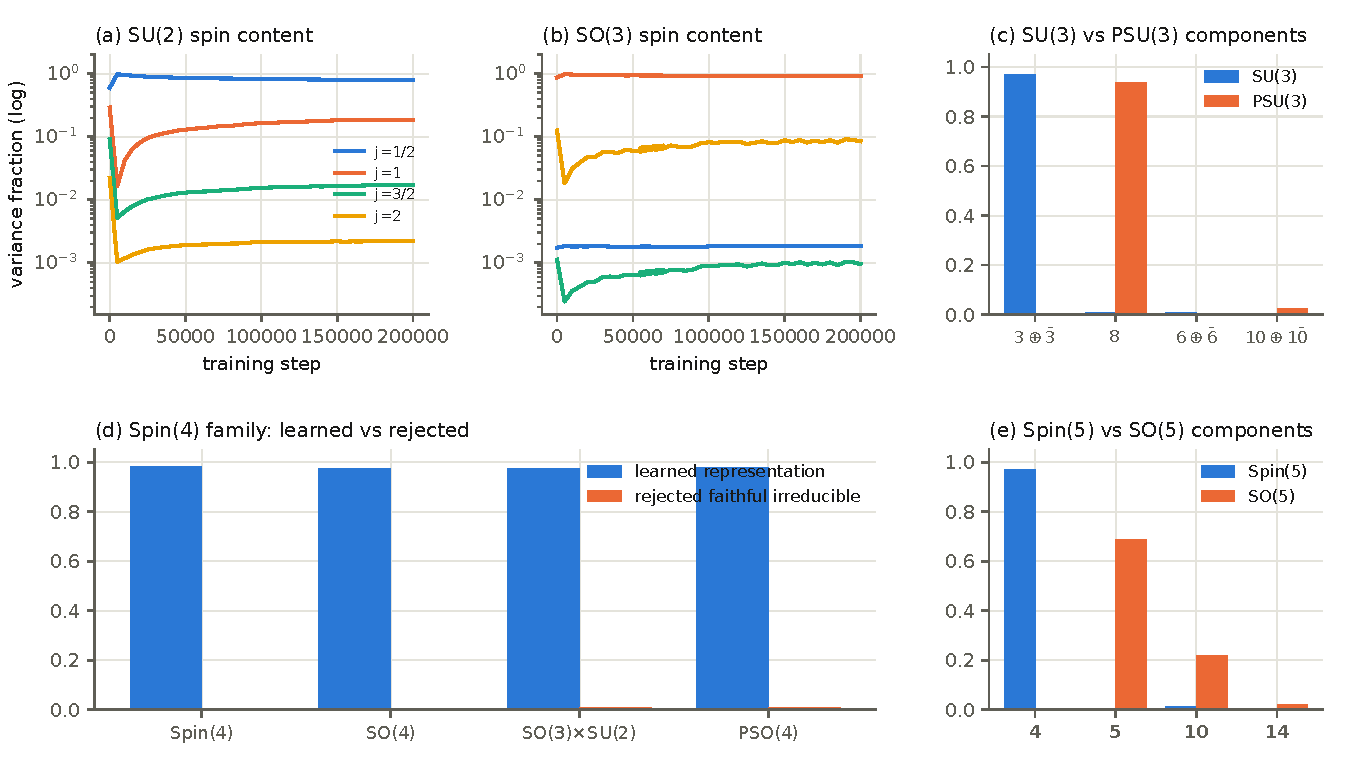
\includegraphics[width=\textwidth]{figureA1.pdf}
\caption{(a, b) Fraction of encoder variance per spin component during
training for the $\SU(2)$ and $\SO(3)$ conditions (seed 0, log scale, with
the dotted floor marking the sampling limit). (c, d, e) Final component
fractions for $\SU(3)$/$\PSU(3)$, the $\Spin(4)$ family, and
$\Spin(5)$/$\SO(5)$ (means over five seeds).}
\label{fig:appendix}
\end{figure}

\begin{table}[t]
\centering
\caption{Seed statistics for the principal conditions (five seeds, mean
$\pm$ standard deviation, evaluated at $100$k steps). $D$ denotes the
center discrimination appropriate to the condition, the probability that
the true product outscores its center translates, with tie value $0.5$
($\SU(2)$/$\SO(3)$) or $1/3$ ($\SU(3)$/$\PSU(3)$).}
\label{tab:seeds}
\scriptsize
\setlength{\tabcolsep}{4pt}
\begin{tabular}{lcccc}
\toprule
 & $\SU(2)$ & $\SO(3)$ & $\SU(3)$ & $\PSU(3)$ \\
\midrule
held-out accuracy & $0.921 \pm 0.003$ & $0.883 \pm 0.003$ & $0.994 \pm 0.001$ & $0.685 \pm 0.020$ \\
learned-representation variance & $0.835 \pm 0.010$ & $0.917 \pm 0.008$ & $0.971 \pm 0.009$ & $0.934 \pm 0.007$ \\
forbidden-component variance & $0.0023 \pm 0.0004$ & $0.0023 \pm 0.0004$ & $0.0059 \pm 0.0004$ & $0.0000$ \\
center cosine & $-0.72 \pm 0.02$ & $+1.000$ & $-0.484 \pm 0.005$ & $+1.000$ \\
coefficient decode $R^2$ & $0.995$ & $0.999$ & $0.978 \pm 0.006$ & $0.699 \pm 0.012$ \\
$D$, intact & $1.0000$ & $0.5000$ & $1.0000$ & $0.3333$ \\
score--character $R^2$ & $0.974 \pm 0.006$ & $0.876 \pm 0.014$ & $0.700$ & \\
\bottomrule
\end{tabular}
\end{table}

\begin{table}[t]
\centering
\caption{Interventions on the argument encoders for the $\SU(2)$ and
$\SO(3)$ conditions (five seeds, mean $\pm$ standard deviation). Task is
ranking accuracy against $63$ excluded Haar negatives (chance $0.016$),
$D_c$ the probability that the true product outscores its antipode (tie
$0.5$).}
\label{tab:su2causal}
\scriptsize
\begin{tabular}{lcccc}
\toprule
 & \multicolumn{2}{c}{$\SU(2)$} & \multicolumn{2}{c}{$\SO(3)$} \\
intervention & task & $D_c$ & task & $D_c$ \\
\midrule
none & $1.000$ & $1.0000 \pm 0.0000$ & $1.000$ & $0.5000$ \\
ablate spin $\tfrac12$ & $0.026 \pm 0.002$ & $0.503 \pm 0.006$ & $1.000 \pm 0.000$ & $0.5000$ \\
ablate spin $1$ & $1.000 \pm 0.000$ & $1.0000$ & $0.027 \pm 0.003$ & $0.5000$ \\
center-orbit average & $0.021$ & $0.498$ & $1.000$ (exact identity) & $0.5000$ \\
random subspace, equal rank & $1.000$ & $1.0000$ & $1.000$ & $0.5000$ \\
\bottomrule
\end{tabular}
\end{table}

\begin{table}[t]
\centering
\caption{Interventions for the $\SU(3)$ and $\PSU(3)$ conditions (five
seeds). $D_\omega$ is the probability that the true product outscores both
of its center translates (tie $1/3$).}
\label{tab:su3causal}
\scriptsize
\begin{tabular}{lcccc}
\toprule
 & \multicolumn{2}{c}{$\SU(3)$} & \multicolumn{2}{c}{$\PSU(3)$} \\
intervention & task & $D_\omega$ & task & $D_\omega$ \\
\midrule
none & $0.998 \pm 0.001$ & $1.000$ & $0.739 \pm 0.019$ & $0.333$ \\
center-orbit average & $0.016 \pm 0.001$ & $0.337 \pm 0.008$ & $0.739$ (exact identity) & $0.333$ \\
remove invariant part & $0.998$ & $1.000$ & $0.015 \pm 0.001$ & $0.333$ \\
ablate $\mathbf{3} \oplus \bar{\mathbf{3}}$ & $0.018 \pm 0.002$ & $0.335$ & $0.733$ & $0.333$ \\
ablate adjoint $\mathbf{8}$ & $0.997$ & $1.000$ & $0.014 \pm 0.003$ & $0.333$ \\
\bottomrule
\end{tabular}
\end{table}

\begin{table}[t]
\centering
\caption{Interventions resolved by summand for the $\Spin(4)$ family
(five seeds, representative cells with seed statistics). $D_L$, $D_R$,
$D_{LR}$ are the discriminations of the three center elements (tie $0.5$).
Each learned summand is necessary for exactly the center elements its
central character detects.}
\label{tab:spin4causal}
\scriptsize
\begin{tabular}{llccc}
\toprule
condition & intervention & task & $D_L$ & $D_R$ \\
\midrule
$\Spin(4)$ & none & $0.997$ & $1.000$ & $1.000$ \\
$\Spin(4)$ & ablate $(\tfrac12, 0)$ & $0.57$ & $0.507 \pm 0.007$ & $1.000 \pm 0.000$ \\
$\Spin(4)$ & ablate $(0, \tfrac12)$ & $0.57$ & $1.000$ & $0.498$ \\
$\SO(4)$ & ablate $(\tfrac12, \tfrac12)$ & $0.017 \pm 0.001$ & $0.489$ & $0.489$ \\
$\SO(3){\times}\SU(2)$ & ablate $(0, \tfrac12)$ & $0.53$ & $0.500$ & $0.493 \pm 0.006$ \\
$\SO(3){\times}\SU(2)$ & ablate $(1, 0)$ & $0.853 \pm 0.036$ & $0.500$ & $1.000$ \\
$\PSO(4)$ & ablate $(1, 0)$ or $(0, 1)$ & $0.809 \pm 0.016$ & $0.500$ & $0.500$ \\
\bottomrule
\end{tabular}
\end{table}

\begin{table}[t]
\centering
\caption{The two-sided translation test on the $\SO(3)$ condition (five
seeds for the trained and random-initialization systems). Left and right
columns are held-out $R^2$ of fitted affine translation operators, hom-$R$
the right-homomorphism defect, and $[L,R]$ the commutator defect, both
relative to activation norm.}
\label{tab:twosided}
\scriptsize
\begin{tabular}{lccccc}
\toprule
feature system & dim & left $R^2$ & right $R^2$ & hom-$R$ & $[L,R]$ \\
\midrule
trained features & $9$ & $0.989 \pm 0.001$ & $0.989 \pm 0.001$ & $0.012$ & $0.012 \pm 0.001$ \\
full coefficient space & $9$ & $1.000$ & $1.000$ & $0.000$ & $0.000$ \\
two-column frame & $6$ & $1.000$ & $0.638$ & $0.526$ & $0.039$ \\
random subspace of coefficients & $6$ & $0.674$ & $0.675$ & $0.411$ & $0.448$ \\
raw encoding & $32$ & $0.992$ & $0.991$ & $0.058$ & $0.073$ \\
random-initialization encoder & $16$ & $0.892 \pm 0.008$ & $0.890 \pm 0.008$ & $0.179$ & $0.160 \pm 0.014$ \\
\bottomrule
\end{tabular}
\end{table}

\begin{table}[t]
\centering
\caption{Frame against coefficient space in matched training on $\SO(3)$
(five seeds per arm, $60$k steps). Norms are Frobenius norms of module
parameters at the end of training.}
\label{tab:cost}
\scriptsize
\begin{tabular}{lcccccc}
\toprule
encoding & accuracy & margin & encoder norm & interaction norm & scorer norm & margin/norm \\
\midrule
frame, $6$ dims & $0.891 \pm 0.002$ & $6.49 \pm 0.05$ & $19.6$ & $11.9$ & $13.7$ & $0.243 \pm 0.002$ \\
coefficients, $9$ dims & $0.889 \pm 0.003$ & $7.29 \pm 0.16$ & $16.7$ & $9.8$ & $12.2$ & $0.319 \pm 0.008$ \\
\bottomrule
\end{tabular}
\end{table}

\begin{table}[t]
\centering
\caption{Recovery of the character expansion of the score per checkpoint
(sequentially orthogonalized profile, model divided by target, with
components beyond spin $2$ at $0.000$ throughout and omitted). The
band-limited target is $\chi_1 + \tfrac12\chi_2$.}
\label{tab:recovery}
\scriptsize
\begin{tabular}{llcccc}
\toprule
target & step & $j = \tfrac12$ & $j = 1$ & $j = \tfrac32$ & $j = 2$ \\
\midrule
$K_t$, $t = 0.3$ & $25$k & $1.13$ & $1.12$ & $0.13$ & $0.81$ \\
$K_t$, $t = 0.3$ & $60$k & $1.05$ & $1.05$ & $1.01$ & $0.07$ \\
$K_t$, $t = 0.1$ & $60$k & $1.47$ & $1.39$ & $1.43$ & $0.00$ \\
$K_t$, $t = 0.05$ & $50$k & $1.81$ & $1.81$ & $1.71$ & $0.12$ \\
$K_t$, $t = 0.05$ & $100$k & $1.63$ & $1.63$ & $1.49$ & $0.83$ \\
$K_t$, $t = 0.05$ & $120$k & $1.58$ & $1.55$ & $1.46$ & $1.20$ \\
band-limited, wd $1.0$ & $60$k & $1.01$ & $1.20$ & $0.00$ & $0.00$ \\
band-limited, wd $0.1$ & $60$k & $1.00$ & $1.01$ & $0.94$ & $0.95$ \\
\bottomrule
\end{tabular}
\end{table}

\end{document}
